
\documentclass[tikz,border=5pt]{standalone}
\usepackage{tikz}
\usepackage{siunitx}
\usetikzlibrary{%
    spath3,
    intersections,
    arrows,
    knots,
    calc,
    hobby,
    decorations.pathreplacing,
    shapes.geometric,
}


\tikzset{
  knot diagram/every strand/.append style={
    ultra thick,
    red
  },
    every path/.style={red,line width=2pt},
    every node/.style={transform shape,knot crossing,inner sep=1.5pt},
    every knot/.style={line cap=round,line join=round,very thick},
    strand/.style={line cap=round,line join=round,line width=3pt,draw=black},
    over/.style={preaction={draw=white,line width=6.5pt}},
}


% Turn guides off when you're happy:
\newif\ifguides
\guidestrue   % ← change to \guidesfalse for final

\begin{document}

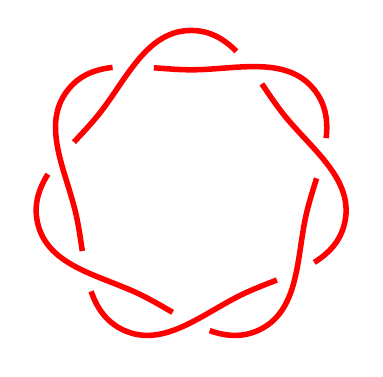
\begin{tikzpicture}[use Hobby shortcut]
\path[spath/save=7-1]
([closed]90:2) foreach \k in {1,...,7} {
  .. (90-360/7+\k*720/7:1.5) .. (90+\k*720/7:2)
} (90:2);
\tikzset{
  every spath component/.style={draw},
  spath/knot={7-1}{15pt}{1,3,...,15}
}
\end{tikzpicture}




\begin{tikzpicture}[line cap=round, line join=round, scale=1.05]
    % Explicit coordinates for 14 interleaved points (odd on R=3.0, even on r=2.0)
    \coordinate (P1)  at (  0,       3      );
    \coordinate (P2)  at ( -0.8678,  1.8019 );
    \coordinate (P3)  at ( -2.3455,  1.8705 );
    \coordinate (P4)  at ( -1.9499,  0.4450 );
    \coordinate (P5)  at ( -2.9248, -0.6676 );
    \coordinate (P6)  at ( -1.5637, -1.2470 );
    \coordinate (P7)  at ( -1.3017, -2.7029 );
    \coordinate (P8)  at (  0,      -2      );
    \coordinate (P9)  at (  1.3017, -2.7029 );
    \coordinate (P10) at (  1.5637, -1.2470 );
    \coordinate (P11) at (  2.9248, -0.6676 );
    \coordinate (P12) at (  1.9499,  0.4450 );
    \coordinate (P13) at (  2.3455,  1.8705 );
    \coordinate (P14) at (  0.8678,  1.8019 );
    \coordinate (P15) at (P1);
%
%    \begin{knot}[
%        consider self intersections,
%        clip width=6pt,
%        clip radius=3pt,
%        ignore endpoint intersections=false,
%        draft mode=crossings,         % <- shows numbers at each crossing
%        flip crossing/.list={1,3}     % <- crossings to put "under"
%    ]
%    \strand
%    ([closed] P1)..(P2)..(P5)..(P6)..(P9)..(P10)..(P13)..(P14)..(P3)..(P4)..(P7)..(P8)..(P11)..(P12)..(P1);
%    \end{knot}

    %
    % =========================================================
    % Guides (circles, dots, labels, skeleton) — turn off with \guidesfalse
    % =========================================================
    \ifguides
    % helper circles
    \draw[gray!35, dashed] (0,0) circle (\Rodd);
    \draw[gray!35, dashed] (0,0) circle (\Reven);
    % points + labels
    \foreach \i/\pos in {1/above,2/above right,3/right,4/right,
    5/below right,6/below,7/below,8/below left,
    9/left,10/left,11/left,12/above left,
    13/above,14/above right}{
        \fill[blue] (P\i) circle (1.4pt);
        \node[blue,\pos,font=\scriptsize] at (P\i) {\i};
    }
    % optional skeleton in index order
    \draw[gray!40, dashed](P1)--(P2)--(P5)--(P6)--(P9)--(P10)--(P13)--(P14)--(P3)--(P4)--(P7)--(P8)--(P11)--(P12)--cycle;
    \fi
\end{tikzpicture}


% Stevedore knot (6_1) in the same style as your 5_2 example
\begin{tikzpicture}[use Hobby shortcut, scale=1.05]
    % ===== hand-tuned points to match your silhouette =====
    % top sweep (low, wide dome)
    \coordinate (P1)  at ( 0,  1.5);
    \coordinate (P2)  at (-2,  2);
    \coordinate (P3)  at (-1.5, 0);
    \coordinate (P4)  at (1, -1.5);
    \coordinate (P5)  at (-1.5, -2);
    \coordinate (P6)  at (-2.5, -0.5);
    \coordinate (P7)  at (-1.5, 1);
    \coordinate (P8)  at ( 0, 3);
    \coordinate (P9)  at ( 1.5, 1);
    \coordinate (P10) at ( 2.5, -0.5);
    \coordinate (P11) at (1.5, -2);
    \coordinate (P12) at (-1,  -1.5);
    \coordinate (P13) at ( 1.5,  0);
    \coordinate (P14) at ( 2,  2);
    \coordinate (P15) at ( 0,  1.5);
    % close near start (must equal P1 for a smooth closed Hobby curve)

    \begin{knot}[
        consider self intersections,
        draft mode=crossings,      % <- shows crossing numbers while tuning
        clip width=5pt,
        clip radius=3pt,
        ignore endpoint intersections=false,
    % Typical alternating over/under for 6_1; adjust if numbering differs:
        flip crossing/.list={1,3,5,7}
    ]
        % Single closed strand: tuned control points to produce the 6_1 (Stevedore)
    \strand
    ([closed] P1)..(P2)..(P3)..(P4)..(P5)..(P6)..(P7)..(P8)..(P9)..(P10)..(P11)..(P12)..(P13)..(P14)..(P15);
    \end{knot}

    \ifguides
% Show handles + skeleton so reshaping is easy
    \foreach \i/\pos in {1/above right,2/right,3/below,4/left,5/left,6/left,7/above,8/right,9/right,10/below right,11/below,12/below left,13/left,14/above left,15/above right}{
        \fill[blue] (P\i) circle (1.2pt);
        \node[blue,\pos,font=\scriptsize] at (P\i) {\i};
    }
    \draw[gray!40, dashed](P1)--(P2)--(P3)--(P4)--(P5)--(P6)--(P7)--(P8)--(P9)--(P10)--(P11)--(P12)--(P13)--(P14)--(P15);
    \fi
\end{tikzpicture}

%  Up Quarck knot (5_2)
\begin{tikzpicture}[use Hobby shortcut, line cap=round, line join=round, scale=1.05]
    % ===== Up Quark knot (5_2): control points =====
    \coordinate (P1) at ( 2.0,  2.0);  % start / close
    \coordinate (P2) at ( 1.8,  0.0);
    \coordinate (P3) at (-2.3, -1.0);
    \coordinate (P4) at ( 0.5,  1.0);
    \coordinate (P5) at (-2.0,  2.0);
    \coordinate (P6) at (-1.8,  0.0);
    \coordinate (P7) at ( 2.3, -1.0);
    \coordinate (P8) at (-0.5,  1.0);
    \coordinate (P9) at ( 2.0,  2.0);  % = P1 (smooth closed path)

    \begin{knot}[
        consider self intersections,
        draft mode=crossings,              % show crossing indices while tuning
        ignore endpoint intersections=false,
        clip width=5pt, clip radius=3pt,
        flip crossing/.list={6,4,2}        % same over/under pattern as your snippet
    ]
    \strand
    ([closed] P1)..(P2)..(P3)..(P4)..(P5)..(P6)..(P7)..(P8)..(P9);
    \end{knot}

    \ifguides
    % Point labels + dashed skeleton for quick reshaping
    \foreach \i/\pos in {1/above right,2/right,3/below left,4/above,5/above left,6/below,7/below right,8/left,9/above right}{
        \fill[blue] (P\i) circle (1.2pt);
        \node[blue,\pos,font=\scriptsize] at (P\i) {\i};
    }
    \draw[gray!40, dashed](P1)--(P2)--(P3)--(P4)--(P5)--(P6)--(P7)--(P8)--(P9);
    \fi
\end{tikzpicture}



% Hopf Link
\begin{tikzpicture}
    \begin{knot}[
    %  draft mode=crossings,
      flip crossing=2
    ]
    \strand (1,0) circle[radius=2cm];
    \strand[blue] (-1,0) circle[radius=2cm];
    \end{knot}
\end{tikzpicture}

% borromean knot
\begin{tikzpicture}
    \begin{knot}[
      draft mode=crossings,
      flip crossing/.list={3,4}
    ]
    \strand (1,0) circle[radius=2cm];
    \strand[blue] (-1,0) circle[radius=2cm];
    \strand[green] (0,{sqrt(3)}) circle[radius=2cm];
    \end{knot}
\end{tikzpicture}



% Septfoil (7_1)
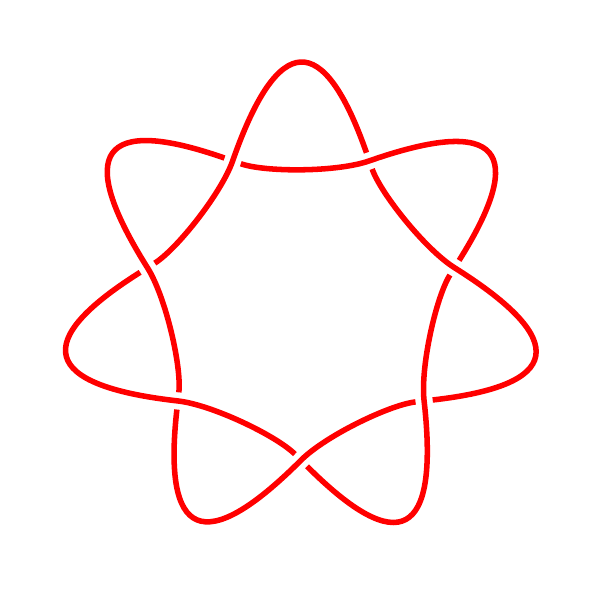
\begin{tikzpicture}
\foreach \brk in {0,...,6} {
    \begin{scope}[rotate=\brk * 51.42857]
    \node (k\brk) at (0,-2) {};
    \end{scope}
}
\draw (0,0) \foreach \brk in {0,...,6} {
    let \n0=\brk,
    \n1={int(Mod(\brk+1,7))},
    \n2={int(Mod(\brk+2,7))}
    in (k\n0) .. controls (k\n0.16 south east) and (k\n1.16 south west) ..
    (k\n1.center) .. controls (k\n1.4 north east) and (k\n2.4 north west) ..
    (k\n2)} (k2);
\end{tikzpicture}


% Cincefoil (5_1)
\begin{tikzpicture}
    \begin{knot}[
      consider self intersections=true,
      draft mode=crossings,
      flip crossing/.list={2,4},
      only when rendering/.style={
        show curve controls
      }
    ]
    \strand (2,0) .. controls +(0,1.0) and +(54:1.0) .. (144:2) .. controls +(54:-1.0) and +(18:-1.0) .. (-72:2) .. controls +(18:1.0) and +(162:-1.0) .. (72:2) .. controls +(162:1.0) and +(126:1.0) .. (-144:2) .. controls +(126:-1.0) and +(0,-1.0) .. (2,0);
    \end{knot}
\end{tikzpicture}

% Figure-8 knot (4_1)
\begin{tikzpicture}[use Hobby shortcut]
    \begin{knot}[
      consider self intersections=true,
      draft mode=crossings,
      ignore endpoint intersections=false,
        flip crossing/.list={1,3,5,7}
      only when rendering/.style={
        show curve endpoints
      }
    ]
    \strand ([closed]0,0) .. (1.5,1) .. (.5,2) .. (-.5,1) .. (.5,0) .. (0,-.5) .. (-.5,0) .. (.5,1) .. (-.5,2) .. (-1.5,1) .. (0,0);
    \end{knot}
    \path (0,-.7);
\end{tikzpicture}

% Trefoil knot (3_1) 3sides blue, 3 side red
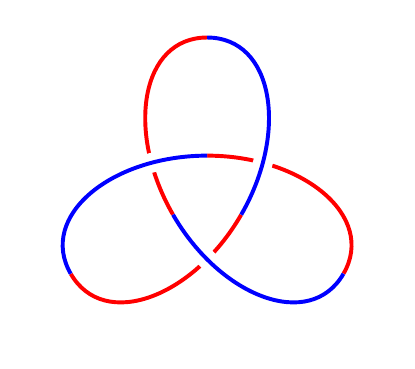
\begin{tikzpicture}[
     use Hobby shortcut,
     every path/.style={
        line width=1mm,
        white,
        double=red,
        double distance=.5mm
     }
    ]
    \def\nfoil{3}
    \draw ([closed]0,2)
    foreach \k in {1,...,\nfoil} {
     .. ([blank=soft]90+360*\k/\nfoil-180/\nfoil:-.5) .. (90+360*\k/\nfoil:2)
    };
    \draw[use previous Hobby path={invert soft blanks,disjoint},double=blue];
\end{tikzpicture}


% Trefoil knot (3_1) 1 side blue, 1 side red
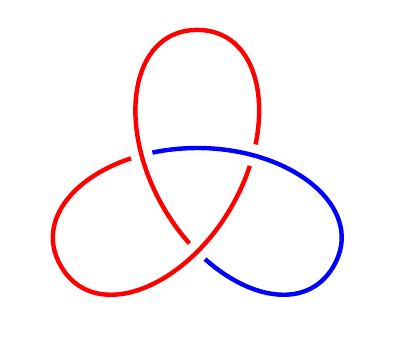
\begin{tikzpicture}[
      use Hobby shortcut,
      every trefoil component/.style={ultra thick, draw, red},
      trefoil component 1/.style={blue},
    ]
    \path[spath/save=trefoil] ([closed]90:2) foreach \k in {1,...,3} { .. (-30+\k*240:.5) .. (90+\k*240:2) } (90:2);
    \tikzset{spath/knot={trefoil}{8pt}{1,3,5}}
\end{tikzpicture}



%---------- Examples of knots ----------

% Trefoil knot (3_1)
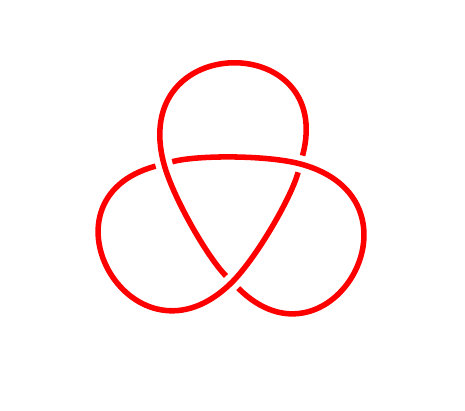
\begin{tikzpicture}
    \foreach \brk in {0,1,2} {
    \begin{scope}[rotate=\brk * 120]
    \node (k\brk) at (0,-1) {};
    \end{scope}
    }
    \draw (0,0) \foreach \brk in {0,1,2} {
        let \n0=\brk,
            \n1={int(Mod(\brk+1,3))},
            \n2={int(Mod(\brk+2,3))}
           in (k\n0) .. controls (k\n0.16 south east) and (k\n1.16 south west) ..
              (k\n1.center) .. controls (k\n1.4 north east) and (k\n2.4 north west) ..
              (k\n2)} (k2);
\end{tikzpicture}

% Cincefoil (5_1)
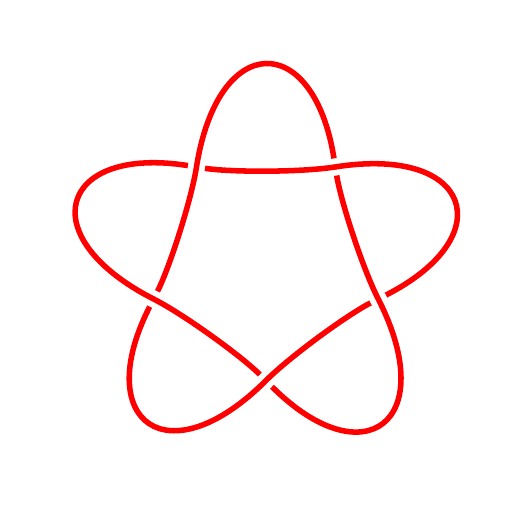
\begin{tikzpicture}
    \foreach \brk in {0,...,4} {
        \begin{scope}[rotate=\brk * 72]
        \node (k\brk) at (0,-1.5) {};
        \end{scope}
    }
    \draw (0,0) \foreach \brk in {0,...,4} {
        let \n0=\brk,
            \n1={int(Mod(\brk+1,5))},
            \n2={int(Mod(\brk+2,5))}
        in (k\n0) .. controls (k\n0.16 south east) and (k\n1.16 south west) ..
           (k\n1.center) .. controls (k\n1.4 north east) and (k\n2.4 north west) ..
           (k\n2)} (k2);
\end{tikzpicture}



% Figure-8 (4_1)
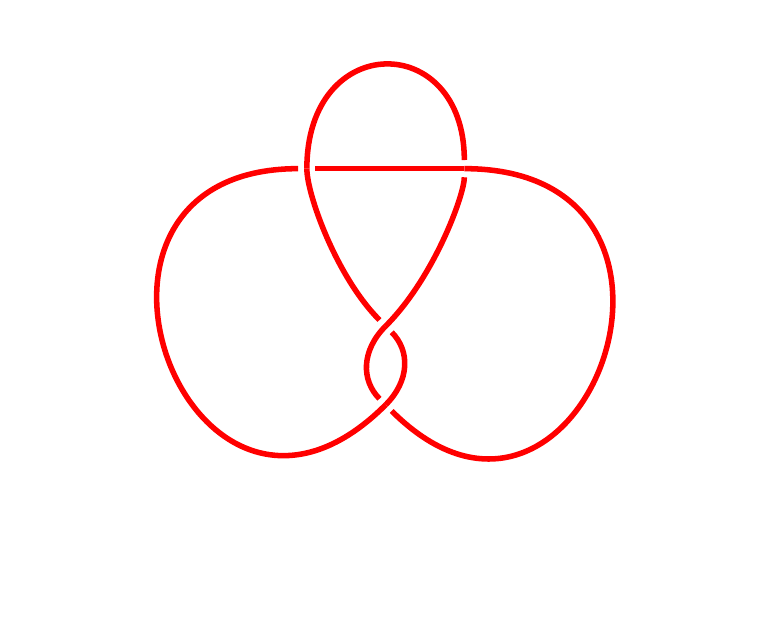
\begin{tikzpicture}
    \node[rotate=45] (tl) at (-1,1) {};
    \node[rotate=-45] (tr) at (1,1) {};
    \edef\twists{1}
    \foreach \brk in {0,...,\twists} {
    \node (m\brk) at (0,-1 - \brk) {};
    }
    \foreach \brk in {1,...,\twists} {
    \pgfmathparse{int(\brk - 1)}
    \edef\brl{\pgfmathresult}
    \draw (m\brk) .. controls (m\brk.4 north west) and (m\brl.4 south west) .. (m\brl.center);
    \draw (m\brk.center) .. controls (m\brk.4 north east) and (m\brl.4 south east) .. (m\brl);
    }
    \draw (m0) .. controls (m0.8 north west) and (tl.3 south west) .. (tl.center);
    \draw (m0.center) .. controls (m0.8 north east) and (tr.3 south east) .. (tr);
    \draw (tl.center) .. controls (tl.16 north east) and (tr.16 north west) .. (tr);
    \draw (m\twists) .. controls (m\twists.32 south east) and (tr.32 north east) .. (tr.center);
    \draw (m\twists.center) .. controls (m\twists.32 south west) and (tl.32 north west) .. (tl);
    \draw (tl) -- (tr.center);
\end{tikzpicture}

\end{document}